% Options for packages loaded elsewhere
\PassOptionsToPackage{unicode}{hyperref}
\PassOptionsToPackage{hyphens}{url}
%
\documentclass[
  10pt,
  ngerman,
  ignorenonframetext,
]{beamer}
\title{AGG - Allgemeines Gleichbehandlungsgesetz}
\subtitle{Seminar: Personalauswahl WiSe 21/22}
\author{Roman Hoehn}
\date{01/03/2022}

\usepackage{pgfpages}
\setbeamertemplate{caption}[numbered]
\setbeamertemplate{caption label separator}{: }
\setbeamercolor{caption name}{fg=normal text.fg}
\beamertemplatenavigationsymbolsempty
% Prevent slide breaks in the middle of a paragraph
\widowpenalties 1 10000
\raggedbottom
\setbeamertemplate{part page}{
  \centering
  \begin{beamercolorbox}[sep=16pt,center]{part title}
    \usebeamerfont{part title}\insertpart\par
  \end{beamercolorbox}
}
\setbeamertemplate{section page}{
  \centering
  \begin{beamercolorbox}[sep=12pt,center]{part title}
    \usebeamerfont{section title}\insertsection\par
  \end{beamercolorbox}
}
\setbeamertemplate{subsection page}{
  \centering
  \begin{beamercolorbox}[sep=8pt,center]{part title}
    \usebeamerfont{subsection title}\insertsubsection\par
  \end{beamercolorbox}
}
\AtBeginPart{
  \frame{\partpage}
}
\AtBeginSection{
  \ifbibliography
  \else
    \frame{\sectionpage}
  \fi
}
\AtBeginSubsection{
  \frame{\subsectionpage}
}
\usepackage{amsmath,amssymb}
\usepackage{lmodern}
\usepackage{iftex}
\ifPDFTeX
  \usepackage[T1]{fontenc}
  \usepackage[utf8]{inputenc}
  \usepackage{textcomp} % provide euro and other symbols
\else % if luatex or xetex
  \usepackage{unicode-math}
  \defaultfontfeatures{Scale=MatchLowercase}
  \defaultfontfeatures[\rmfamily]{Ligatures=TeX,Scale=1}
\fi
\usetheme[]{Szeged}
\usecolortheme{beaver}
% Use upquote if available, for straight quotes in verbatim environments
\IfFileExists{upquote.sty}{\usepackage{upquote}}{}
\IfFileExists{microtype.sty}{% use microtype if available
  \usepackage[]{microtype}
  \UseMicrotypeSet[protrusion]{basicmath} % disable protrusion for tt fonts
}{}
\makeatletter
\@ifundefined{KOMAClassName}{% if non-KOMA class
  \IfFileExists{parskip.sty}{%
    \usepackage{parskip}
  }{% else
    \setlength{\parindent}{0pt}
    \setlength{\parskip}{6pt plus 2pt minus 1pt}}
}{% if KOMA class
  \KOMAoptions{parskip=half}}
\makeatother
\usepackage{xcolor}
\IfFileExists{xurl.sty}{\usepackage{xurl}}{} % add URL line breaks if available
\IfFileExists{bookmark.sty}{\usepackage{bookmark}}{\usepackage{hyperref}}
\hypersetup{
  pdftitle={AGG - Allgemeines Gleichbehandlungsgesetz},
  pdfauthor={Roman Hoehn},
  pdflang={de-DE},
  hidelinks,
  pdfcreator={LaTeX via pandoc}}
\urlstyle{same} % disable monospaced font for URLs
\newif\ifbibliography
\usepackage{color}
\usepackage{fancyvrb}
\newcommand{\VerbBar}{|}
\newcommand{\VERB}{\Verb[commandchars=\\\{\}]}
\DefineVerbatimEnvironment{Highlighting}{Verbatim}{commandchars=\\\{\}}
% Add ',fontsize=\small' for more characters per line
\usepackage{framed}
\definecolor{shadecolor}{RGB}{248,248,248}
\newenvironment{Shaded}{\begin{snugshade}}{\end{snugshade}}
\newcommand{\AlertTok}[1]{\textcolor[rgb]{0.94,0.16,0.16}{#1}}
\newcommand{\AnnotationTok}[1]{\textcolor[rgb]{0.56,0.35,0.01}{\textbf{\textit{#1}}}}
\newcommand{\AttributeTok}[1]{\textcolor[rgb]{0.77,0.63,0.00}{#1}}
\newcommand{\BaseNTok}[1]{\textcolor[rgb]{0.00,0.00,0.81}{#1}}
\newcommand{\BuiltInTok}[1]{#1}
\newcommand{\CharTok}[1]{\textcolor[rgb]{0.31,0.60,0.02}{#1}}
\newcommand{\CommentTok}[1]{\textcolor[rgb]{0.56,0.35,0.01}{\textit{#1}}}
\newcommand{\CommentVarTok}[1]{\textcolor[rgb]{0.56,0.35,0.01}{\textbf{\textit{#1}}}}
\newcommand{\ConstantTok}[1]{\textcolor[rgb]{0.00,0.00,0.00}{#1}}
\newcommand{\ControlFlowTok}[1]{\textcolor[rgb]{0.13,0.29,0.53}{\textbf{#1}}}
\newcommand{\DataTypeTok}[1]{\textcolor[rgb]{0.13,0.29,0.53}{#1}}
\newcommand{\DecValTok}[1]{\textcolor[rgb]{0.00,0.00,0.81}{#1}}
\newcommand{\DocumentationTok}[1]{\textcolor[rgb]{0.56,0.35,0.01}{\textbf{\textit{#1}}}}
\newcommand{\ErrorTok}[1]{\textcolor[rgb]{0.64,0.00,0.00}{\textbf{#1}}}
\newcommand{\ExtensionTok}[1]{#1}
\newcommand{\FloatTok}[1]{\textcolor[rgb]{0.00,0.00,0.81}{#1}}
\newcommand{\FunctionTok}[1]{\textcolor[rgb]{0.00,0.00,0.00}{#1}}
\newcommand{\ImportTok}[1]{#1}
\newcommand{\InformationTok}[1]{\textcolor[rgb]{0.56,0.35,0.01}{\textbf{\textit{#1}}}}
\newcommand{\KeywordTok}[1]{\textcolor[rgb]{0.13,0.29,0.53}{\textbf{#1}}}
\newcommand{\NormalTok}[1]{#1}
\newcommand{\OperatorTok}[1]{\textcolor[rgb]{0.81,0.36,0.00}{\textbf{#1}}}
\newcommand{\OtherTok}[1]{\textcolor[rgb]{0.56,0.35,0.01}{#1}}
\newcommand{\PreprocessorTok}[1]{\textcolor[rgb]{0.56,0.35,0.01}{\textit{#1}}}
\newcommand{\RegionMarkerTok}[1]{#1}
\newcommand{\SpecialCharTok}[1]{\textcolor[rgb]{0.00,0.00,0.00}{#1}}
\newcommand{\SpecialStringTok}[1]{\textcolor[rgb]{0.31,0.60,0.02}{#1}}
\newcommand{\StringTok}[1]{\textcolor[rgb]{0.31,0.60,0.02}{#1}}
\newcommand{\VariableTok}[1]{\textcolor[rgb]{0.00,0.00,0.00}{#1}}
\newcommand{\VerbatimStringTok}[1]{\textcolor[rgb]{0.31,0.60,0.02}{#1}}
\newcommand{\WarningTok}[1]{\textcolor[rgb]{0.56,0.35,0.01}{\textbf{\textit{#1}}}}
\usepackage{graphicx}
\makeatletter
\def\maxwidth{\ifdim\Gin@nat@width>\linewidth\linewidth\else\Gin@nat@width\fi}
\def\maxheight{\ifdim\Gin@nat@height>\textheight\textheight\else\Gin@nat@height\fi}
\makeatother
% Scale images if necessary, so that they will not overflow the page
% margins by default, and it is still possible to overwrite the defaults
% using explicit options in \includegraphics[width, height, ...]{}
\setkeys{Gin}{width=\maxwidth,height=\maxheight,keepaspectratio}
% Set default figure placement to htbp
\makeatletter
\def\fps@figure{htbp}
\makeatother
\setlength{\emergencystretch}{3em} % prevent overfull lines
\providecommand{\tightlist}{%
  \setlength{\itemsep}{0pt}\setlength{\parskip}{0pt}}
\setcounter{secnumdepth}{-\maxdimen} % remove section numbering
\newlength{\cslhangindent}
\setlength{\cslhangindent}{1.5em}
\newlength{\csllabelwidth}
\setlength{\csllabelwidth}{3em}
\newlength{\cslentryspacingunit} % times entry-spacing
\setlength{\cslentryspacingunit}{\parskip}
\newenvironment{CSLReferences}[2] % #1 hanging-ident, #2 entry spacing
 {% don't indent paragraphs
  \setlength{\parindent}{0pt}
  % turn on hanging indent if param 1 is 1
  \ifodd #1
  \let\oldpar\par
  \def\par{\hangindent=\cslhangindent\oldpar}
  \fi
  % set entry spacing
  \setlength{\parskip}{#2\cslentryspacingunit}
 }%
 {}
\usepackage{calc}
\newcommand{\CSLBlock}[1]{#1\hfill\break}
\newcommand{\CSLLeftMargin}[1]{\parbox[t]{\csllabelwidth}{#1}}
\newcommand{\CSLRightInline}[1]{\parbox[t]{\linewidth - \csllabelwidth}{#1}\break}
\newcommand{\CSLIndent}[1]{\hspace{\cslhangindent}#1}
\ifXeTeX
  % Load polyglossia as late as possible: uses bidi with RTL langages (e.g. Hebrew, Arabic)
  \usepackage{polyglossia}
  \setmainlanguage[]{german}
\else
  \usepackage[main=ngerman]{babel}
% get rid of language-specific shorthands (see #6817):
\let\LanguageShortHands\languageshorthands
\def\languageshorthands#1{}
\fi
\ifLuaTeX
  \usepackage{selnolig}  % disable illegal ligatures
\fi

\begin{document}
\frame{\titlepage}

\begin{frame}[allowframebreaks]
  \tableofcontents[hideallsubsections]
\end{frame}
\hypertarget{rechtliche-grundlagen}{%
\section{Rechtliche Grundlagen}\label{rechtliche-grundlagen}}

\begin{frame}{Rechtliche Grundlagen}
\begin{figure}
\centering

\includegraphics{plots/fig1.png}
\caption{Wordcloud
de.wikipedia.org/wiki/Allgemeines\_Gleichbehandlungsgesetz}
\end{figure}
\end{frame}

\begin{frame}{Hintergrund}
\protect\hypertarget{hintergrund}{}
Ein allgemeines Benachteiligungsverbot wird Bürgern der Bundesrepublik
seit 1949 durch Art.3. Abs.3 des Grundgesetzes garantiert:

\begin{quote}
``Niemand darf wegen seines Geschlechtes, seiner Abstammung, seiner
Rasse, seiner Sprache, seiner Heimat und Herkunft, seines Glaubens,
seiner religiösen oder politischen Anschauungen benachteiligt oder
bevorzugt werden. Niemand darf wegen seiner Behinderung benachteiligt
werden.'' (\protect\hyperlink{ref-gg}{\emph{GG}, 1949}, Paragraph 3,
Abs. 3)
\end{quote}

Zahlreiche weitere Reglungen zum Grundsatz der Gleichbehandlung
existieren u.a. in den folgenden Gesetzen:

\begin{itemize}
\tightlist
\item
  BGB
\item
  BetrVG
\item
  Sozialgesetzbuch
\item
  ArbGG
\end{itemize}
\end{frame}

\begin{frame}{Erlassung allgemeines Gleichbehandlungsgesetzes}
\protect\hypertarget{erlassung-allgemeines-gleichbehandlungsgesetzes}{}
\begin{itemize}
\item
  Das AGG wird im Jahre 2006 erlassen
\item
  Zielsetzung: Grundsatz der Gleichbehandlung und Bekämpfung von
  Diskriminierung soll einheitlich und im Einklang mit europäischen
  Richtlinien reguliert werden
\item
  Rechtsfolgen aus dem Gesetzt für multiple Rechtsgebiete:

  \begin{enumerate}
  \tightlist
  \item
    \textbf{Arbeitsrecht}
  \item
    Zivilrecht
  \item
    Soldatenrecht
  \item
    Sozialrecht
  \end{enumerate}
\end{itemize}

(\protect\hyperlink{ref-main}{Rühl, M., 2008}, Seite 17)
\end{frame}

\begin{frame}{Geschützter Personenkreis}
\protect\hypertarget{geschuxfctzter-personenkreis}{}
Das AGG schützt im arbeitsrechtlichen Kontext einen sehr weiten Kreis
von Personen, insbesondere:

\begin{enumerate}
\tightlist
\item
  Arbeitnehmer/-innen (abhängige Beschäftigungsverhältnisse)
\item
  Auszubildende
\item
  Arbeitnehmerähnliche Personen (wirtschaftlich unselbstständige)
\end{enumerate}

\emph{Zusätzlich werden auch Bewerber/-innen und ehemalige Beschäftigte
in den Kreis der geschützten Personen einbezogen}

(\protect\hyperlink{ref-agg}{\emph{AGG}, 2006}, Paragraph 6, Abs 1)
\end{frame}

\begin{frame}{Überblick Geltungsbereich}
\protect\hypertarget{uxfcberblick-geltungsbereich}{}
\begin{figure}
\centering
\includegraphics[width=\textwidth,height=0.75\textheight]{plots/geschützteMerkmale.jpg}
\caption{Geltungsbereich AGG,§1}
\end{figure}
\end{frame}

\begin{frame}{Geschützte Charakteristika}
\protect\hypertarget{geschuxfctzte-charakteristika}{}
Gesetztesziel: Verhinderung und Beseitigung von (arbeitsrechtlichen)
Benachteiligungen aufgrund der folgenden Charakteristika:

\begin{itemize}
\tightlist
\item
  Rasse,
\item
  ethnischer Herkunft,
\item
  Geschlechts,
\item
  Religion,
\item
  Weltanschauung,
\item
  Behinderungen.
\item
  Alters,
\item
  sexuellen Identität
\end{itemize}

\emph{Schützenswert sind die Charakteristika, die von einer Person nicht
beeinflusst werden können (Ausnahme Religion/ Weltanschauung, diese sind
jedoch durch das Grundgesetz geschützt)}

(\protect\hyperlink{ref-agg}{\emph{AGG}, 2006}, Paragraph 1)
\end{frame}

\hypertarget{zahlen-und-statistiken}{%
\section{Zahlen und Statistiken}\label{zahlen-und-statistiken}}

\begin{frame}{Überblick Merkmalsverteilung}
\protect\hypertarget{uxfcberblick-merkmalsverteilung}{}
\begin{figure}
\centering
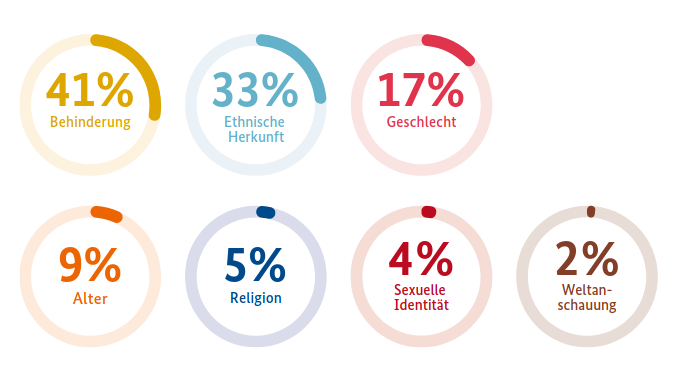
\includegraphics[width=\textwidth,height=0.4\textheight]{plots/verteilung_merkmale_s44.png}
\caption{Übersicht AGG bezogener Beratungsanfragen an die
Antidiskriminierungsstellen im Jahr 2020}
\end{figure}

(\protect\hyperlink{ref-jb2020}{\emph{Jahresbericht 2020}, 2021}, Seite
44)
\end{frame}

\begin{frame}{Überblick jährlicher Beratungsanfragen}
\protect\hypertarget{uxfcberblick-juxe4hrlicher-beratungsanfragen}{}
\begin{figure}
\centering
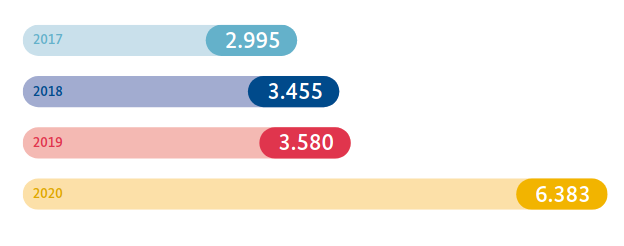
\includegraphics[width=\textwidth,height=0.4\textheight]{plots/entwicklung_beratungsanfragen_agg_s43.png}
\caption{Entwicklung AGG bezogener Beratungsanfragen an die
Antidiskriminierungsstellen 2017-2020}
\end{figure}

(\protect\hyperlink{ref-jb2020}{\emph{Jahresbericht 2020}, 2021}, Seite
43)
\end{frame}

\begin{frame}{Entwicklung jährlicher Beratungsanfragen}
\protect\hypertarget{entwicklung-juxe4hrlicher-beratungsanfragen}{}
\begin{figure}
\centering
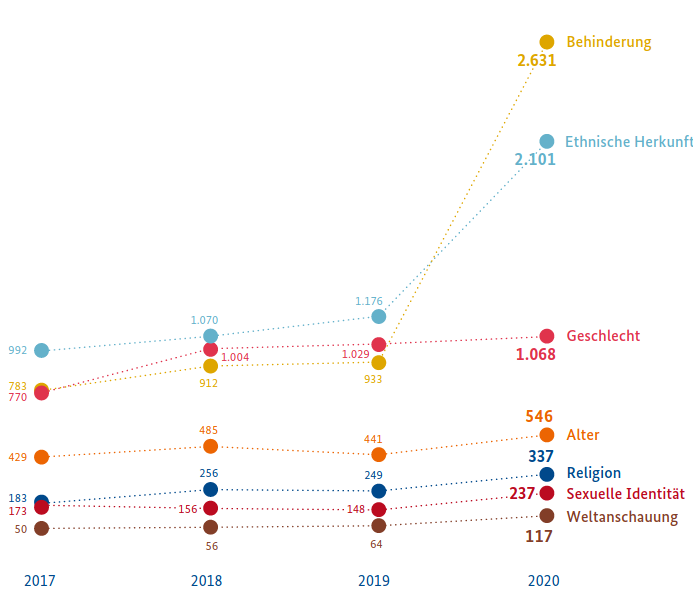
\includegraphics[width=\textwidth,height=0.5\textheight]{plots/entwicklung_beratungsanfragen_nach_merkmalen_s45.png}
\caption{Entwicklung AGG bezogener Beratungsanfragen an die
Antidiskriminierungsstellen 2017-2020, aufgeschlüsselt nach betroffenen
Merkmalen}
\end{figure}

(\protect\hyperlink{ref-jb2020}{\emph{Jahresbericht 2020}, 2021}, Seite
45)
\end{frame}

\hypertarget{formen-der-benachteiligung}{%
\section{Formen der Benachteiligung}\label{formen-der-benachteiligung}}

\begin{frame}{Überblick Benachteiligungen}
\protect\hypertarget{uxfcberblick-benachteiligungen}{}
\begin{figure}
\centering
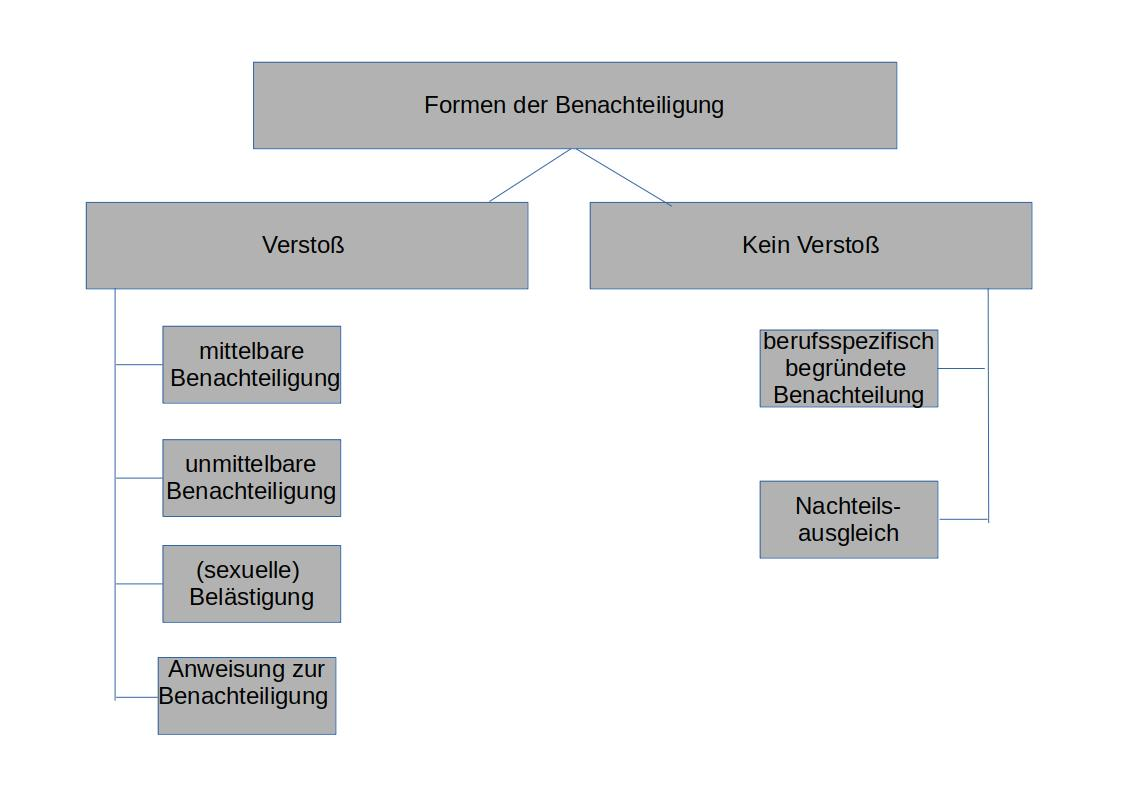
\includegraphics[width=\textwidth,height=0.75\textheight]{plots/benachteiligung.jpg}
\caption{Formen der Benachteiligung}
\end{figure}
\end{frame}

\begin{frame}{Formen der Benachteiligung (2/3)}
\protect\hypertarget{formen-der-benachteiligung-23}{}
\begin{block}{Unmittelbare Benachteiligung}
\protect\hypertarget{unmittelbare-benachteiligung}{}
Die benachteiligte Person erfährt eine weniger günstige Behandlung im
\textbf{Vergleich} zu anderen Personen.
(\protect\hyperlink{ref-agg}{\emph{AGG}, 2006}, Paragraph 3, Satz 1)
\end{block}

\begin{block}{Mittelbare Benachteiligung}
\protect\hypertarget{mittelbare-benachteiligung}{}
Vorschriften, Kriterien oder Verfahren \textbf{könnten} eine Person
benachteiligen (\protect\hyperlink{ref-agg}{\emph{AGG}, 2006}, Paragraph
3, Satz 2)

Es ist notwendig, dass die Benachteiligung aufgrund eines oder mehreren
der geschützten Charakteristika aus Paragraph 1 auftreten.
\end{block}
\end{frame}

\begin{frame}{Formen der Benachteiligung (3/3) -}
\protect\hypertarget{formen-der-benachteiligung-33--}{}
\begin{block}{Benachteiligung durch Belästigungen und/oder sexuelle
Belästigung}
\protect\hypertarget{benachteiligung-durch-beluxe4stigungen-undoder-sexuelle-beluxe4stigung}{}
Unerwünschte Verhaltensweisen, die potentiell die Würde des Empfängers
verletzten könnten (\protect\hyperlink{ref-agg}{\emph{AGG}, 2006},
Paragraph 3, Satz 3,4) -
\end{block}

\begin{block}{Anweisungen zur Benachteiligung}
\protect\hypertarget{anweisungen-zur-benachteiligung}{}
Die Abgabe von Anweisungen, die eine Benachteiligung einer Person nach
sich ziehen könnte (mittelbar oder unmittelbar), werden gleichgestellt
direkten Ausführung einer solchen Benachteiligung
(\protect\hyperlink{ref-agg}{\emph{AGG}, 2006}, Paragraph 3, Satz 5)
\end{block}
\end{frame}

\begin{frame}{Zulässige Benachteiligung}
\protect\hypertarget{zuluxe4ssige-benachteiligung}{}
In bestimmten Fällen, ist es für Arbeitgeber zulässig, Personen aufgrund
von geschützten Charakteristika zu benachteiligen:

\begin{block}{Spezifische berufliche Anforderungen}
\protect\hypertarget{spezifische-berufliche-anforderungen}{}
Für die Ausübung einer spezifischen beruflichen Tätigkeit, stellen die
geschützten Charakteristika ein wesentliches Hindernis dar
(\protect\hyperlink{ref-agg}{\emph{AGG}, 2006}, Paragraph 8)

\begin{itemize}
\tightlist
\item
  Bsp.: Altersgrenzen bei der Einstellung von Feuerwehrsleuten
\item
  Bsp.: Körperliche Belastbarkeit in Handwerksberufen
\end{itemize}
\end{block}

\begin{block}{Nachteilsausgleichende Maßnahmen}
\protect\hypertarget{nachteilsausgleichende-mauxdfnahmen}{}
Gezielten Förderung von benachteiligten Gruppe
(\protect\hyperlink{ref-agg}{\emph{AGG}, 2006}, Paragraph 5)

\begin{itemize}
\tightlist
\item
  Bsp.: Bevorzugte Einstellung von Schwerbehinderten
\item
  Bsp.: Frauenförderung
\end{itemize}
\end{block}
\end{frame}

\hypertarget{fallbeispiel}{%
\section{Fallbeispiel}\label{fallbeispiel}}

\begin{frame}{Fallbeispiel}
\begin{block}{Fall 1}
\protect\hypertarget{fall-1}{}
Ein katholischer Bewerber wird im Auswahlverfahren um die Stelle für die
Leitung eines jüdischen Museums aufgrund seiner Religionszugehörigkeit
abgelehnt.
\end{block}

\begin{block}{Fall 2}
\protect\hypertarget{fall-2}{}
Eine Bewerberin mit Legasthenie wird bei der Auswahl für eine
Lektoratsstelle aufgrund ihrer Einschränkung ausgeschlossen.

\emph{Zulässig oder Verstoß gegen das AGG ?}
\end{block}
\end{frame}

\hypertarget{arbeitsrechtliche-umsetzung}{%
\section{Arbeitsrechtliche
Umsetzung}\label{arbeitsrechtliche-umsetzung}}

\begin{frame}{Unternehmerische Konsequenzen}
\protect\hypertarget{unternehmerische-konsequenzen}{}
Bewerber/-Innen und Mitarbeiter/-Innen können Schadensansprüche gegen
Organisation geltend machen, sofern Sie eine Ungleichbehandlung
nachweisen können.(\protect\hyperlink{ref-agg}{\emph{AGG}, 2006},
Paragraph 15)

\begin{itemize}
\tightlist
\item
  Ein üblicher Schadensersatzanspruch beläuft sich auf ca. 3
  Bruttogehälter der angestrebten Stelle
\end{itemize}

\emph{Zusätzliche Gefahr des ``AGG Hoppings'', systematische Verwertung
von AGG Verstößen durch Schadensersatzansprüche}
\end{frame}

\begin{frame}[fragile]{Rechenbeispiel}
\protect\hypertarget{rechenbeispiel}{}
100 Bewerber/-Innen bewerben sich auf eine Stellenanzeige mit einem
Frauen-benachteiligendem Ausschreibungstext. Das monatliche Bruttogehalt
für die Stelle beläuft sich auf 3000€.

Potentielle Schadensersatzzahlungen bei Klage von 50 Bewerberinnen:

\begin{Shaded}
\begin{Highlighting}[]
\NormalTok{(}\DecValTok{3000} \SpecialCharTok{*} \DecValTok{3}\NormalTok{) }\SpecialCharTok{*} \DecValTok{50}
\end{Highlighting}
\end{Shaded}

\begin{verbatim}
== [1] 450000
\end{verbatim}

\emph{Zusätzlich können nicht unerhebliche Kosten für die rechtliche
Vertretung auf das Unternehmen zukommen}
\end{frame}

\begin{frame}{Vorbeugende Maßnahmen und Pflichten des AG}
\protect\hypertarget{vorbeugende-mauxdfnahmen-und-pflichten-des-ag}{}
Generalklausel: Arbeitgeber sollen durch geeignete Maßnahmen,
beispielsweise Aus- und Fortbildung, der Ungleichbehandlung von
geschützen Personen entgegenwirken
(\protect\hyperlink{ref-agg}{\emph{AGG}, 2006}, Paragraph 12, Abs.1)

\textbf{Es besteht eine Pflicht für den AG entsprechende Maßnahmen
umzusetzen!}

Präventive Maßnahmen umfassen z.B.:

\begin{itemize}
\tightlist
\item
  Diversity Training
\item
  Rechtliche Schulungen
\item
  Sensibilisierungstrainings (z.B. gegen Mobbing)
\end{itemize}

Informationsmaßnahmen:

\begin{itemize}
\tightlist
\item
  Aushang des Gesetzestexts
\item
  AGG konforme Leitfäden
\item
  Ansprechpartner im Unternehmen
\end{itemize}
\end{frame}

\begin{frame}{Auswirkungen auf die Personalbeschaffung}
\protect\hypertarget{auswirkungen-auf-die-personalbeschaffung}{}
Um arbeitsrechtliche Verstöße zu vermeiden, müssen Unternehmen ihre
Personalbeschaffungsmaßnahmen AGG konform implementieren. Kritisch sind
insbesondere zwei Bereiche der Personalbeschaffung:

\begin{itemize}
\tightlist
\item
  \textbf{Personalwerbung}: An die gewünschten Bewerber/-Innen
  gerichtete Informations-, Kommunikations- und Aktivierungsmaßnahmen
\item
  \textbf{Personalauswahl}: Analyse und Auswahl von Bewerber/-Innen
  anhand ihres Eignungspotentials für das Unternehmen
\end{itemize}

(\protect\hyperlink{ref-woehe}{Wöhe, 2013}, Seite 129)
\end{frame}

\begin{frame}{Personalwerbung - Stellenausschreibungen}
\protect\hypertarget{personalwerbung---stellenausschreibungen}{}
Die Ausschreibung von Stellen, sowohl intern als auch extern, muss
sorgfältig formuliert werden um nicht gegen das AGG zu verstoßen
\end{frame}

\begin{frame}{Geschlechtsneutrale Formulierung}
\protect\hypertarget{geschlechtsneutrale-formulierung}{}
\textbf{Empfehlenswerte Vorgehensweisen}:

\begin{itemize}
\tightlist
\item
  ausschließlich Funktionsbezeichnugen nennen, z.B. Abteilungsleitung
\item
  explizite Nennung von Männlich/Weiblich/Divers
\item
  juristische Expertise einholen
\end{itemize}

\textbf{Exemplarische Verstöße}:

\begin{itemize}
\tightlist
\item
  Ausschreibung einer Stelle als Krankenschwester
\item
  Stellenbezeichnung im generisches Maskulinum, z.B. ``Abteilungsleiter
  gesucht''
\end{itemize}

Selbst scheinbar harmlose Formulierungen, wie ``Vollzeitstelle'' oder
``Körperliche Belastbarkeit vorausgesetzt'' können und wurden bereits
als Verstöße gegen das AGG kategorisiert.

(\protect\hyperlink{ref-ihk_wsb}{Scheibig, B., o.~J.})
\end{frame}

\begin{frame}{Altersdiskriminierunde Formulierungen}
\protect\hypertarget{altersdiskriminierunde-formulierungen}{}
Formulierungen können sowohl jüngere als auch ältere Bewerber
benachteiligen:

\begin{itemize}
\tightlist
\item
  ``Unser junges und dynamisches Team sucht Verstärkung''
\item
  ``Langjährige Berufserfahrung wird vorausgesetzt''
\end{itemize}

Altersgrenzen müssen vermieden werden, wenn diese nicht aus besonderen
beruflichen Gründen gerechtfertigt sind.

(\protect\hyperlink{ref-ihk_wsb}{Scheibig, B., o.~J.})
\end{frame}

\begin{frame}{Weitere diskriminierende Formulierungen}
\protect\hypertarget{weitere-diskriminierende-formulierungen}{}
Zahlreiche weitere Formulierungen können gegen das AGG verstoßen

\begin{itemize}
\tightlist
\item
  ``körperlich uneingeschränkt leistungsfähiger Vetriebsleiter gesucht''

  \begin{itemize}
  \tightlist
  \item
    Diskriminierung von körperlich behinderten Bewerbern
  \end{itemize}
\item
  ``Englischer Muttersprachler für unser Dolmetscherbüro gesucht''

  \begin{itemize}
  \tightlist
  \item
    Diskriminierung von Menschen anderer Herkunft
    (\protect\hyperlink{ref-ihk_wsb}{Scheibig, B., o.~J.})
  \end{itemize}
\end{itemize}
\end{frame}

\begin{frame}{Personalauswahl}
\protect\hypertarget{personalauswahl}{}
\begin{itemize}
\item
  Bei der Auswahl von Kandidaten aus dem Bewerberpool müssen Unternehmen
  ebenfalls darauf achten keine Verstöße gegen das AGG zu begehen.
\item
  Empfehlungen:

  \begin{itemize}
  \tightlist
  \item
    Klare Definition von (nicht diskriminierenden) Auswahlkriterien
  \item
    Transparentes und nachvollziehbares Verfahren
  \item
    Lückenlose Dokumentation des Prozesses
  \end{itemize}
\end{itemize}

(\protect\hyperlink{ref-ihk_wsb}{Scheibig, B., o.~J.})
\end{frame}

\begin{frame}{Auswahlkriterien}
\protect\hypertarget{auswahlkriterien}{}
Das Festlegen von nicht-diskriminierenden Auswahlkriterien ist Grundlage
einer AGG konformen Personalauswahl:

\begin{itemize}
\tightlist
\item
  berufliche Qualifikationen
\item
  Aus- und Weiterbildungsstatus
\item
  Sprach- oder EDV Kenntnisse
\end{itemize}

AGG Verstöße drohen hingegen bei Ausschluss von Bewerben aufgrund von:

\begin{itemize}
\tightlist
\item
  fehlendem Bewerbungsfoto
\item
  fehlender Angabe des Geburtsdatums
\item
  unvollständiger Angabe des Namens (z.B. nur Vorname angegeben)
\item
  Vorhandensein von Kindern
\end{itemize}

(\protect\hyperlink{ref-ihk_wsb}{Scheibig, B., o.~J.})
\end{frame}

\begin{frame}{Dokumentationsempfehlungen (1/3)}
\protect\hypertarget{dokumentationsempfehlungen-13}{}
Falls das Unternehmen beschuldigt wird, einen Bewerber ungleich
behandelt zu haben, muss das Unternehmen diese Beschuldigung aktiv
widerlegen.

Als wichtigste Verteidigungslinie gilt die lückenlose Dokumentation
aller Phasen und Entscheidungen der Personalauswahl.

Anmerkung: Die umfassende Dokumentation und Aufbewahrung ist rechtlich
nicht verpflichtend vorgeschrieben.
\end{frame}

\begin{frame}{Dokumentationsempfehlung (2/3)}
\protect\hypertarget{dokumentationsempfehlung-23}{}
Die Dokumentation sollte folgende Punkte umfassen:

\begin{enumerate}
\tightlist
\item
  Nach welchen Kriterien wurden eingehende Bewerbungen evaluiert?
\item
  Archivierung von Kopien aller eingegangenen Bewerbungen (potentielle
  Beweismittel)\footnote<.->{Orginale dürfen nach Ablehung des Bewerbers
    nichts archiviert werden.}
\item
  Protokollierung von Bewerbungsgesprächen
\end{enumerate}

Anmerkung: Bewerber müssen ihre Ansprüche bei AGG Verstößen innerhalb
einer Frist von 2 Monaten geltend machen. Für Bewerbungsunterlagen
gelten daher vergleichsweise kurze Aufbewahrungszeiten.
\end{frame}

\begin{frame}[fragile]{Dokumentationsempfehlung (3/3)}
\protect\hypertarget{dokumentationsempfehlung-33}{}
\textbf{Besondere sorgfältige Dokumentation muss bei dem Ausschluss von
Bewerbern aus dem Auswahlverfahren erfolgen}:

\begin{verbatim}
* Auf welcher Entscheidungsgrundlage ist der Teilnehmer ausgeschlossen worden?
* In welcher Phase des Verfahrens ist der Teilnehmer ausgeschlossen worden?
\end{verbatim}

(\protect\hyperlink{ref-ihk_wsb}{Scheibig, B., o.~J.})
\end{frame}

\begin{frame}{Take Home Message}
\protect\hypertarget{take-home-message}{}
\begin{enumerate}
\tightlist
\item
  Das AGG schützt im arbeitsrechtlichen Kontext Arbeitnehmer,
  Auftragsnehmer, Auszubildenden sowie Bewerber und ehemalige
  Beschäftigte
\item
  Durch das AGG geschützte Merkmale umfassen: - Rasse \& ethnischer
  Herkunft, - Geschlechts \& sexuelle Identität, - Religion,
  Weltanschauung, - Alter \& Behinderungen.
\item
  Verstöße gegen das AGG können sowohl mittelbar als auch unmittelbar
  geschehen
\item
  Ungleichbehandlungen sind zulässig, sofern Sie beruflich gerechtfertig
  sind oder dem Nachteilsausgleich dienen
\item
  Personalwerbung: Starke Sorgfalt und juristische / personalpolitische
  Expertise bei der Formulierung
\item
  Personalauswahl: Lückenlose Dokumentation als rechtlicher Schutz gegen
  Anschuldigungen
\end{enumerate}
\end{frame}

\hypertarget{literaturverzeichnis}{%
\section*{Literaturverzeichnis}\label{literaturverzeichnis}}
\addcontentsline{toc}{section}{Literaturverzeichnis}

\begin{frame}{Literaturverzeichnis}
\hypertarget{refs}{}
\begin{CSLReferences}{1}{0}
\leavevmode\vadjust pre{\hypertarget{ref-agg}{}}%
\emph{AGG: Allgemeines Gleichbehandlungsgesetz}. (2006).

\leavevmode\vadjust pre{\hypertarget{ref-gg}{}}%
\emph{GG: Grundgesetz der Bundesrepublik Deutschland}. (1949).

\leavevmode\vadjust pre{\hypertarget{ref-jb2020}{}}%
\emph{Jahresbericht 2020: Jahresbericht der Antidiskriminierungsstelle
des Bundes}. (2021). Antidiskriminierungsstelle des Bundes.

\leavevmode\vadjust pre{\hypertarget{ref-main}{}}%
Rühl, M., H. J. (2008). \emph{Das AGG in der Unternehmenspraxis: Wie
Unternehmen und Personalf{ü}hrung Gesetz und Richtlinien rechtssicher
und diskriminierungsfrei umsetzten}. Betriebswirtschaftlicher Verlag
Dr.Th.Gabler.

\leavevmode\vadjust pre{\hypertarget{ref-ihk_wsb}{}}%
Scheibig, B., B. F. (o.~J.). \emph{AGG bei Stellenausschreibungen und
Bewerbungsverfahren: online, abgerufen am 14.12.2021} (Nr. 3553). IHK
Wiesbaden.
\url{https://www.ihk-wiesbaden.de/recht/rechtsberatung/personal/auswirkungen-des-gleichbehandlungsgesetzes-agg-auf-stellenaussc-1255690}

\leavevmode\vadjust pre{\hypertarget{ref-woehe}{}}%
Wöhe, G. (2013). \emph{Einf{ü}hrung in die Allgemeine
Betriebswirtschaftslehre} (25. Auflage). Franz Vahlen.

\end{CSLReferences}
\end{frame}

\end{document}
